\chapter{Execution of Story Diagrams} \label{sec:Execution}

In general, there are two possibilities to execute models: Executing them directly using an interpreter \cite{GHS09} or generating GPL code, which is either compiled or interpreted.

\fuj can generate Java or C code from story diagrams and their accompanying class diagrams. 
Here, a story diagram describes the behavior of a single method. 
Therefore, this method and its containing class must be defined first.

Interpreting a story diagram does not impose this restriction.
In the following sections, we describe the structure and operation principles of an interpreter for story diagrams.


\section{Interpreting Story Diagrams}
\label{sec:InterpretingStoryDiagrams}

\subsection{Interpreter Architecture}

\begin{figure}[htbp]
  \centering
  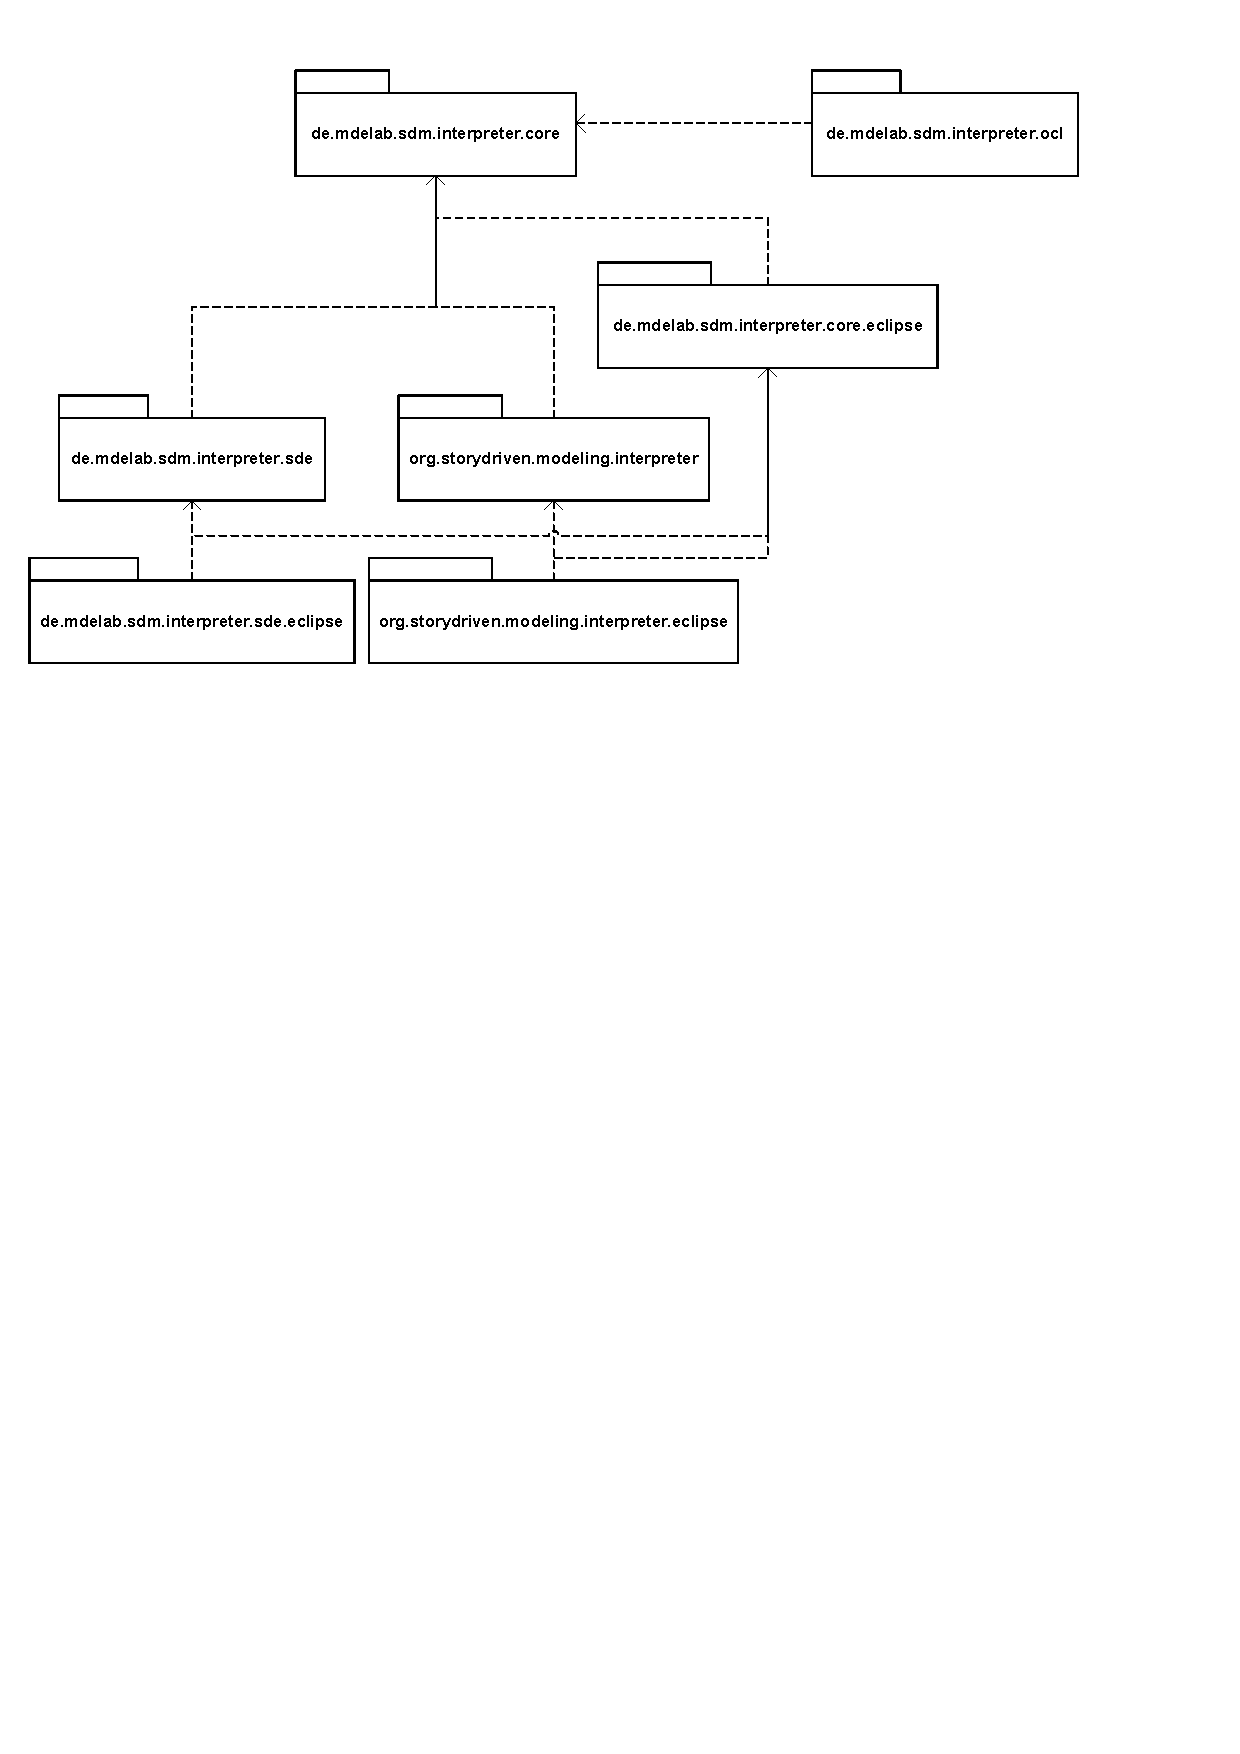
\includegraphics[width=1.0\columnwidth]{./figures/interpreter_packages.pdf}
  \caption{Overview of the Packages of the Interpreter}
  \label{fig:interpreter_packages}
\end{figure}

Figure~\ref{fig:interpreter_packages} shows the package structure of the story diagram interpreter.
Currently, there are multiple story diagram metamodels in use that must all be supported by the interpreter. 
Therefore, the interpreter is divided into a metamodel-independent core (\emph{de.mdelab.sdm.interpreter.core}) and multiple metamodel-dependent extensions (\emph{org.storydriven.modeling.interpreter} and \emph{de.mdelab.sdm.interpreter.sde}). 
This separation of metamodel-dependent and independent parts allows for easier maintenance of the interpreter. 
The classes of the core package define a quite extensive list of generic type parameters (not shown in the subsequent class diagrams), e.g., for activity nodes, classifiers, or features. 
Subclasses in the metamodel-dependent packages replace these generic types with the concrete types defined in the respective metamodel.

Furthermore, those parts of the interpreter that depend on Eclipse are also separated (\emph{*.eclipse} packages). 
This allows to use the interpreter in stand-alone applications without Eclipse. 
In addition, the interpreters for expression languages like OCL are also separated (\emph{de.mdelab.sdm.interpreter.ocl}). 
The story diagram interpreter provides an extension mechanism to add interpreters for other expression languages.
The Eclipse-specific plug-ins provide the additional functionality that expression languages and interpreters for them are registered automatically using an extension point.
Otherwise, the registration of expression languages must be performed explicitly by the interpreter user.
This is the only difference between the core and the Eclipse-based plug-ins.
Therefore, the \emph{*Eclipse} classes will not be explained in detail in the following sections.


\subsubsection{Story Diagram Interpreter}
\label{sec:sdm_interpreter}

\begin{figure}[htbp]
  \centering
  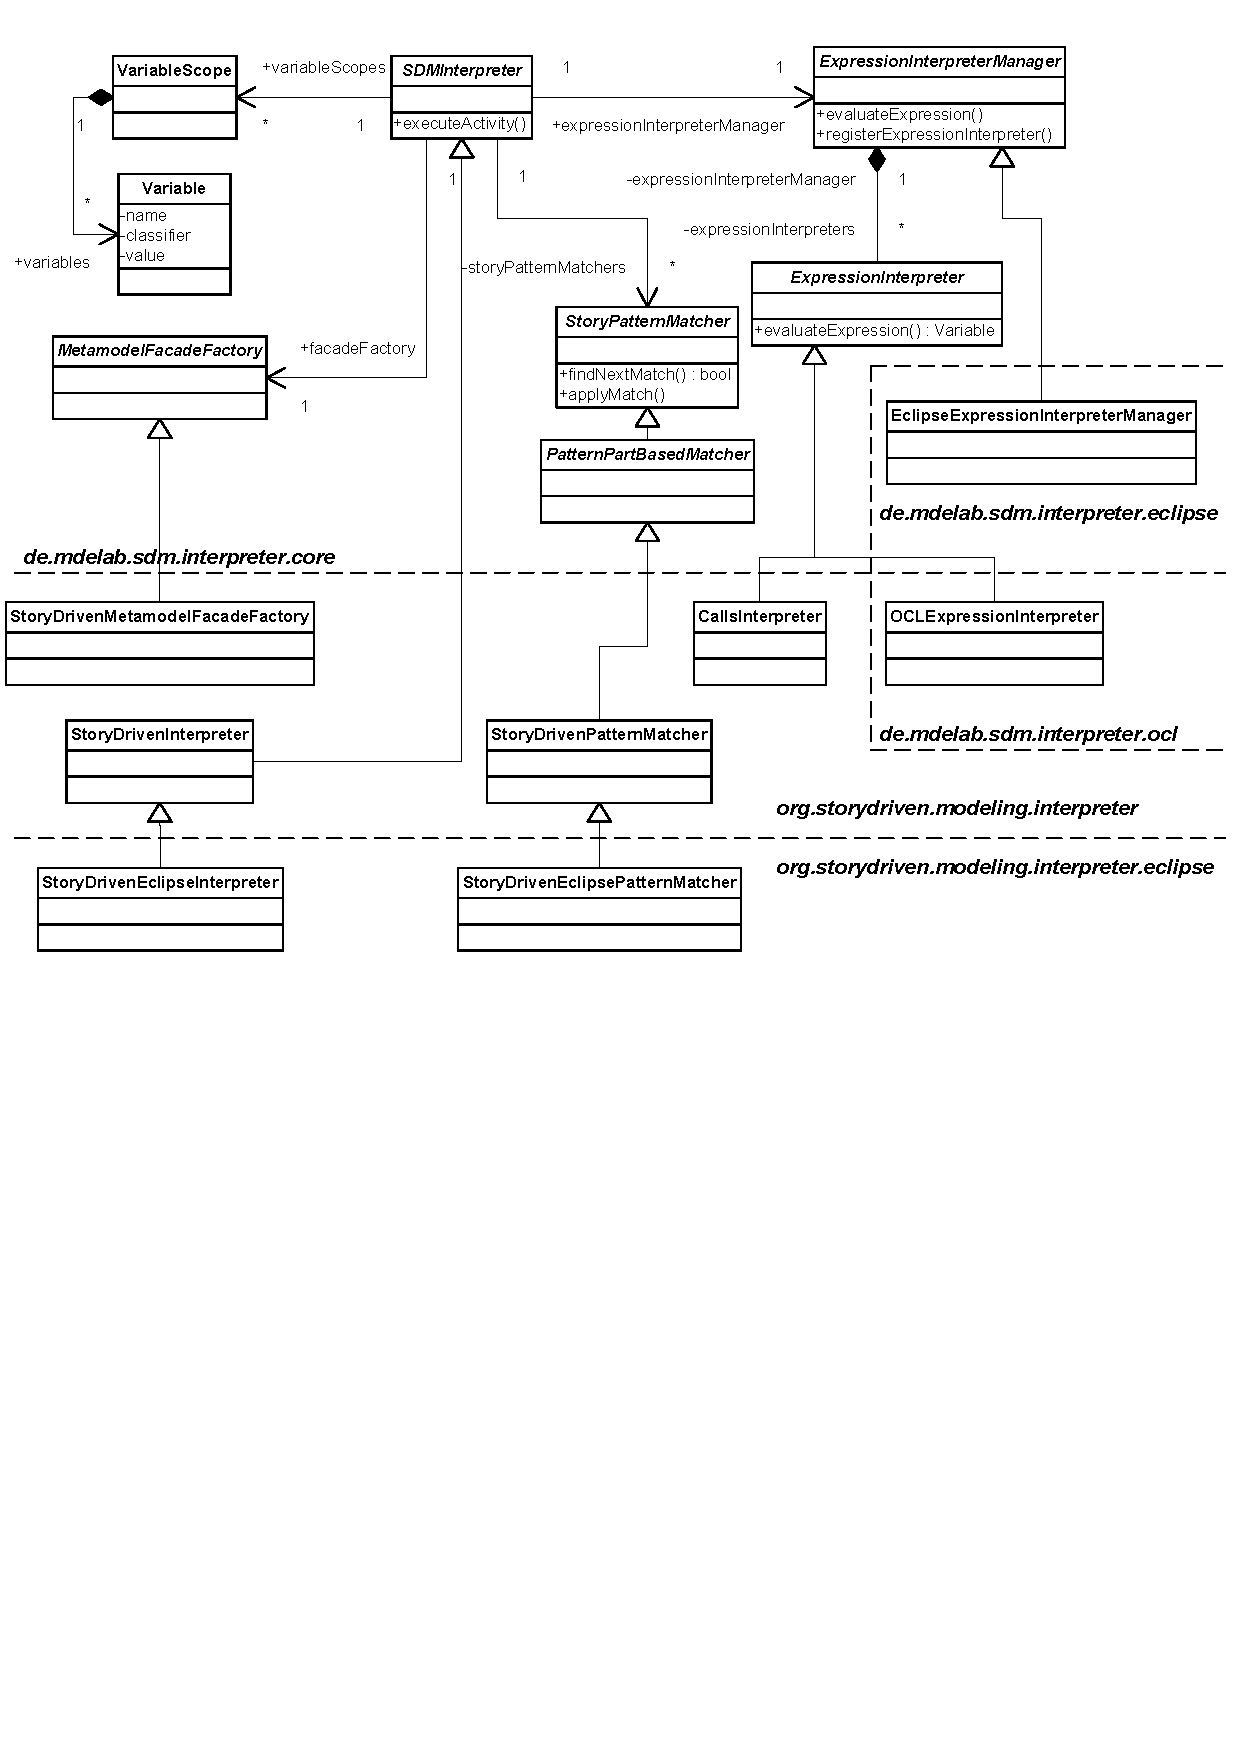
\includegraphics[width=1.0\columnwidth]{./figures/interpreter_core.pdf}
  \caption{Main classes of the interpreter core}
  \label{fig:sdm_interpreter}
\end{figure}

Figure~\ref{fig:sdm_interpreter} shows the main classes of the interpreter core. 
\emph{SDMInterpreter} is the abstract superclass of all story diagram interpreters. 
It is responsible for the execution of a whole story diagram. 
\emph{StoryDrivenInterpreter} and \emph{StoryDrivenEclipseInterpreter} inherit from it to narrow the generic type parameters of \emph{SDMInterpreter} to the specific types of the particular metamodel. 
The \emph{SDMInterpreter} provides the \emph{executeActivity()} method to execute a story diagram.

A \emph{VariableScope} is a collection of \emph{Variable}s that are valid in a specific scope.
A \emph{Variable} is a triple of the name, the classifier, and the value of the variable.
The \emph{SDMInterpreter} maintains multiple \emph{VariableScope}s, one for each activity node.
%\footnote{Currently, the whole story diagram forms a single scope.
%All variables created in a story diagram are also valid in the whole story diagram. 
%Therefore, the same scope is used for all activity nodes.
%Only, when other story diagrams are called, a new variable scope is created. 
%However, if additional elements are added to story diagrams, e.g., fork and join nodes, or if the semantics of existing elements is changed, it is easily possible to support separate scopes for each activity node.}

The \emph{ExpressionInterpreterManager} is responsible for managing the interpreters for expression languages and delegating the evaluation of an expression to the appropriate \emph{ExpressionInterpreter}. 
The \emph{evaluateExpression()} method is provided for that purpose. 
Subclasses of \emph{ExpressionInterpreter}s have to be registered at the \emph{ExpressionInterpreterManager} via the \emph{registerExpressionInterpreter()} method before expressions of that language can be handled, e.g., the \emph{OCLExpressionInterpreter} has to be registerd for OCL expressions before OCL expressions in a story diagram can be evaluated.
Similarly, the \emph{CallsInterpreter} is registered for Calls.
The \emph{EclipseExpressionInterpreterManager} performs this registration automatically. 
The plug-in \emph{de.mdelab.sdm.interpreter.eclipse} defines an extension point for \emph{ExpressionInterpreter}s. 
All interpreters extending this extension point are registered automatically by the \emph{EclipseExpressionInterpreterManager}. 
If the interpreter is not used within Eclipse, \emph{ExpressionInterpreter}s have to be registered explicitly before executing a story diagram.

The abstract class \emph{ExpressionInterpreter} only defines the \emph{evaluateExpression()} method that must be implemented by subclasses such as the \emph{OCLExpressionInterpreter} and the \emph{CallsInterpreter}. 
The method performs the execution of the expression, which may have side effects, and has to return a \emph{Variable} with the return type and return value of the expression. 
In this method, the current \emph{VariableScope} can also be accessed and modified so that variables of the story diagram can be used in expressions.

The interpreter often needs to access specific properties of story diagram elements, e.g., the name of elements or incoming and outgoing edges of activity nodes.
While the interpreter core is metamodel-independent, it cannot access these properties directly but needs a facade for that purpose.
The \emph{MetamodelFacadeFactory} provides access to these facades. 
There are several interfaces for common kinds of story diagram elements (e.g., story nodes, junction nodes, object variables or link variables), which have to be implemented for specific story diagram metamodels.
Subclasses of \emph{MetamodelFacadeFactory} create the facades for the specific story diagram metamodel.

A \emph{StoryPatternMatcher} is responsible for the execution of a single story pattern. 
This abstract superclass defines the methods \emph{findNextMatch()} to search for the next match of a story pattern and \emph{applyMatch()} to execute the graph transformation rule's side effects on the last match. 
The class \emph{StoryPatternMatcher} does not implement a particular matching strategy, i.e., a particular algorithm how to search for matches of the pattern. 
This is done by \emph{PatternPartBasedPatternMatcher}. 
This pattern matching strategy is explained in more detail in Section~\ref{sec:story_pattern_matcher}. 


\subsubsection{Story Pattern Matcher}
\label{sec:story_pattern_matcher}

\begin{figure}[htbp]
  \centering
  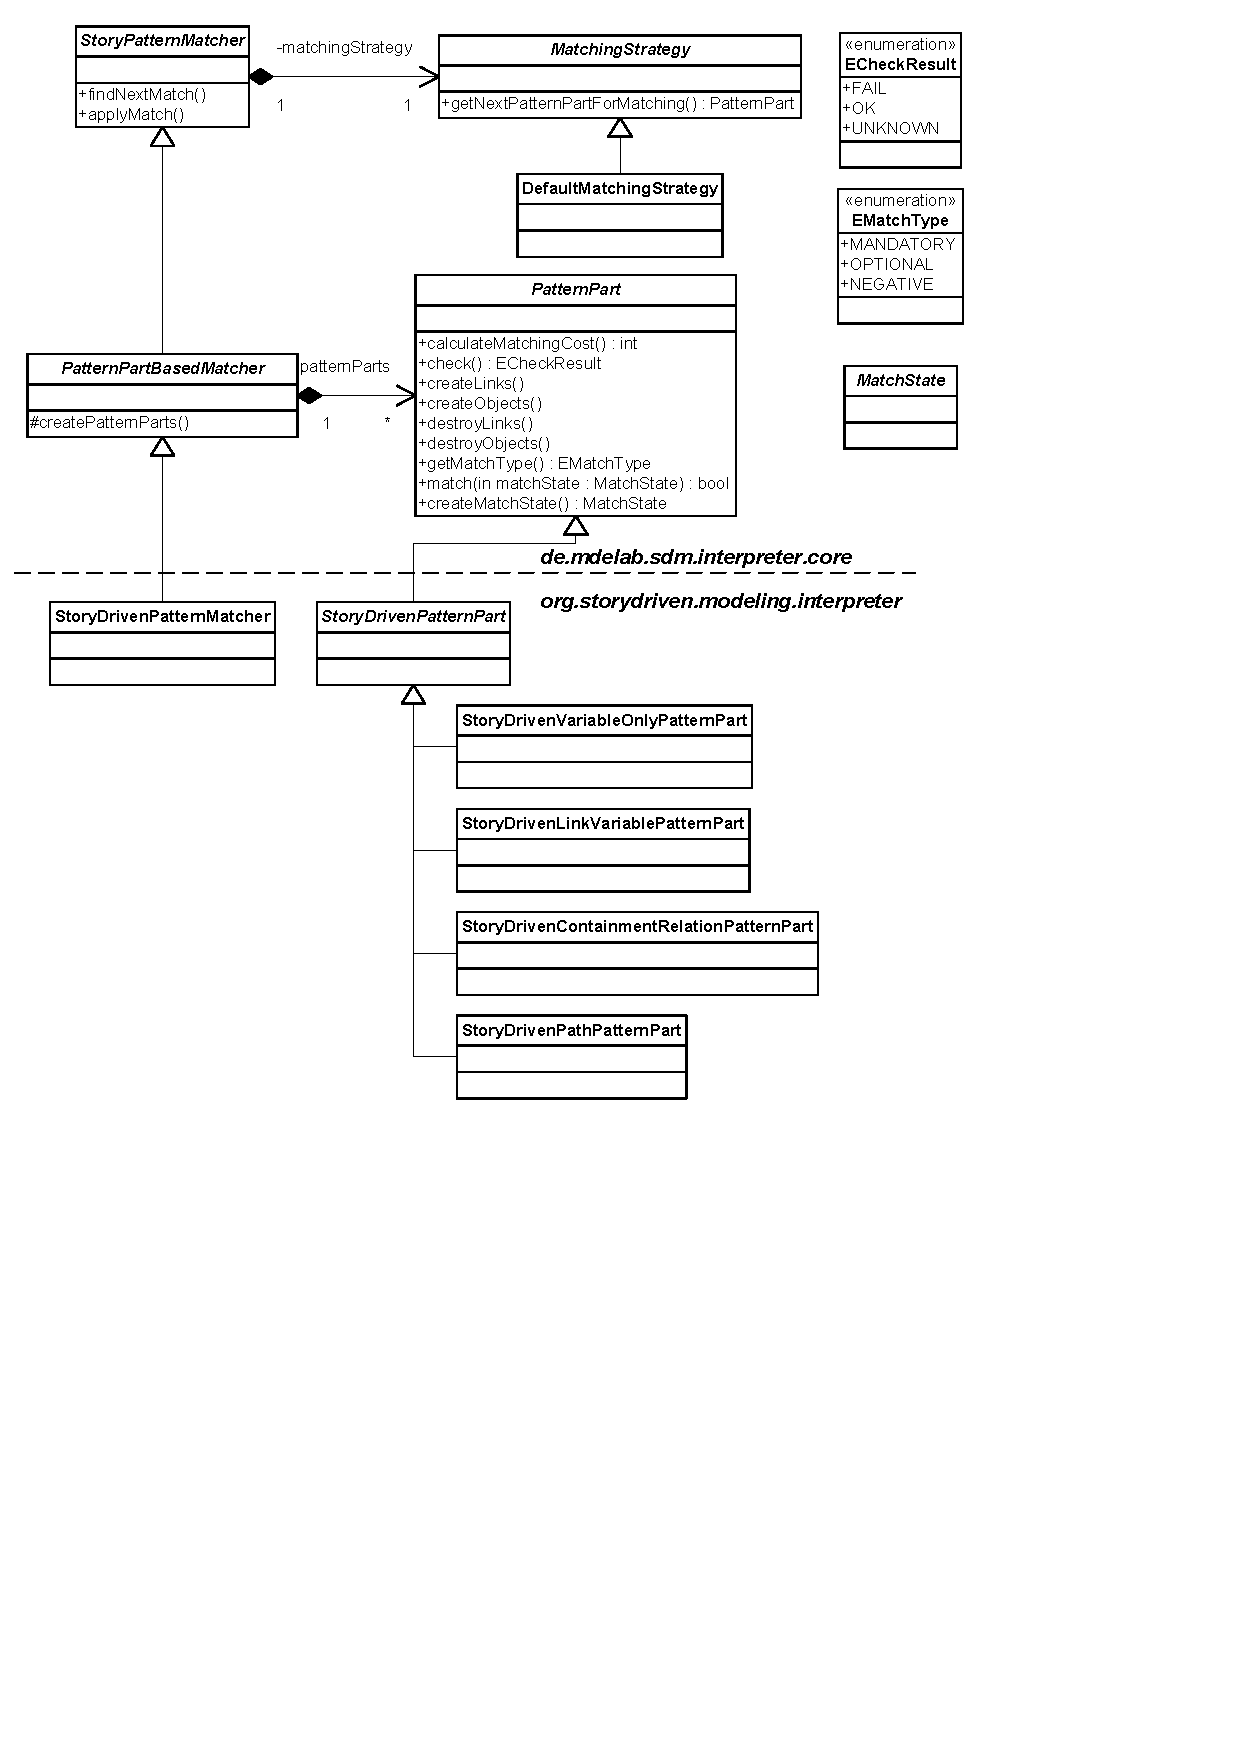
\includegraphics[width=1.0\columnwidth]{./figures/interpreter_storyPatternMatcher.pdf}
  \caption{Main classes of the story pattern matcher}
  \label{fig:interpreter_storyPatternMatcher}
\end{figure}

Figure~\ref{fig:interpreter_storyPatternMatcher} shows the classes of the story pattern matcher. 
Currently, only one pattern matching strategy is implemented. 
The \emph{PatternPartBasedPatternMatcher} splits the story pattern into multiple \emph{PatternPart}s. 
What exactly constitutes a \emph{PatternPart} is not specified in the interpreter core. 
This has to be implemented in the metamodel specific subclasses. 
Currently, the \emph{StoryDrivenPatternMatcher} enforces the following semantics: A pattern part consists either of a single variable that has no incoming or outgoing links (\emph{VariableOnlyPatternPart}), or of a single link and its adjacent object variables (\emph{StoryDrivenLinkVariablePatternPart}, \emph{StoryDrivenContainmentRelationPatternPart}, and \emph{StoryDrivenPathPatternPart} depending on the kind of link). 
This implies that a variable can be contained in more than one pattern parts. 
This semantics can also be modified to support, e.g., complex application conditions or subpatterns, which form a distinct subunit of the pattern.
But this remains transparent to the basic \emph{PatternPartBasedPatternMatcher}.
\emph{MatchState}s are used by \emph{PatternPart}s to temporarily store information about the current matching state, e.g., the iterator of a link to improve performance.
Subclasses are specific for pattern parts and have to define appropriate attributes, e.g., fields for iterator objects.
More information can be found in Sec.~\ref{sec:spm_pattern_matching}.

The \emph{MatchingStrategy} determines the order in which pattern parts are matched. 
The \emph{DefaultMatchingStrategy} matches pattern parts in the order of their matching cost estimates, i.e., \emph{getNextPatternPartForMatching()} returns that pattern part with the lowest cost estimate. 

There are also two additional pattern matching strategies: \emph{DefaultMatchingStrategyWithLog} and \emph{LogReproducingMatchingStrategy}. 
These are required for \emph{for-each} story nodes. For more information, see Sec.~\ref{sec:sdm_interpreting}.

\emph{PatternPart} defines several abstract methods:

\begin{enumerate}
	\item \emph{getMatchType()} returns whether matching the pattern parts is mandatory or optional, or whether the pattern part is a negative application condition (cf. Section~\ref{sec:StoryPatterns:binding:semantics}). 
	
	\item \emph{check()} checks whether the link exists in the instance graph, which requires that all variables of the pattern part are already bound to an instance object. 
	If this is not the case, \emph{check()} returns \emph{UNKNOWN}. 

	\item \emph{calculateMatchingCost()} provides an estimate of the cost to match a variable using the link of the pattern part. 
	This estimate can be based, e.g., on the number of elements contained in the link.
	If it is currently not possible to match this pattern part (e.g., because all variables of the pattern part are still unbound), \emph{-1} is returned.
	This operation is called by the \emph{MatchingStrategy} to select the \emph{PatternPart} that the pattern matcher should use to match the next variable.

	\item \emph{createMatchState()} creates a \emph{MatchState} object that is by the \emph{match()} operation to store information about the matching process.

	\item \emph{match(MatchState matchState)} implements the pattern matching for this kind of pattern part. 
	It is called after \emph{calculateMatchingCost()}. 
	To find a match, at least one variable of the pattern part has to be bound and at least one has to be unbound. 
	Then, \emph{match()} tries to find matches for all unbound variables. 
	This part of the pattern matching algorithm is highly implementation specific. 
	It is not only different for different metamodels,
	it also has to be implemented differently for different kinds of link variables.
	For example, matching an object via an ordinary \emph{LinkVariable} has to be done differently than matching via a \emph{Path} or a \emph{ContainmentRelation}.
	However, this also allows to exploit certain features of the metamodel to improve execution performance. 
	For example, \emph{StoryDrivenContainmentRelationPatternPart} uses EMF's \emph{eContainer()} method to navigate containment links in the opposite direction.	
	The \emph{matchState} parameter can be used to store information about the matching process, e.g., the iterator object of the link.
	
	\item \emph{createLinks()} and \emph{createObjects()} create those elements of the pattern part, that are marked with \create.
	
	\item \emph{destroyLinks()} and \emph{destroyObjects()} destroy links and objects. 
	In contrast to the creation of elements, these steps are separated to ensure an orderly deletion of story pattern variables in the \emph{VariableScope}.
	\footnote{Background: There are two ways to execute story patterns with deleted elements: Destroy all links first and then all objects, or the other way round. 
	EMF also supports unidirectional references. 
	Therefore, deleting objects as implemented in \emph{EcoreUtil.delete()} is done by going from the deleted object to the root of the containment hierarchy (usually the \emph{Resource} or \emph{ResourceSet}) and searching for cross-references to the deleted object. 
	If the links are deleted first when the story pattern is executed, the destroyed object may be removed from its containment hierarchy (if a destroyed link represents this containment). 
	After that, existing cross-references to the destroyed object that are not represented by a link in the story pattern (remember that story patterns have SPO semantics) cannot be found and deleted. 
	For this reason, the interpreter first deletes all objects and then all links.}
	

\end{enumerate}



\subsubsection{Notification Mechanism}
\label{sec:notification_mechanism}

\begin{figure}[htbp]
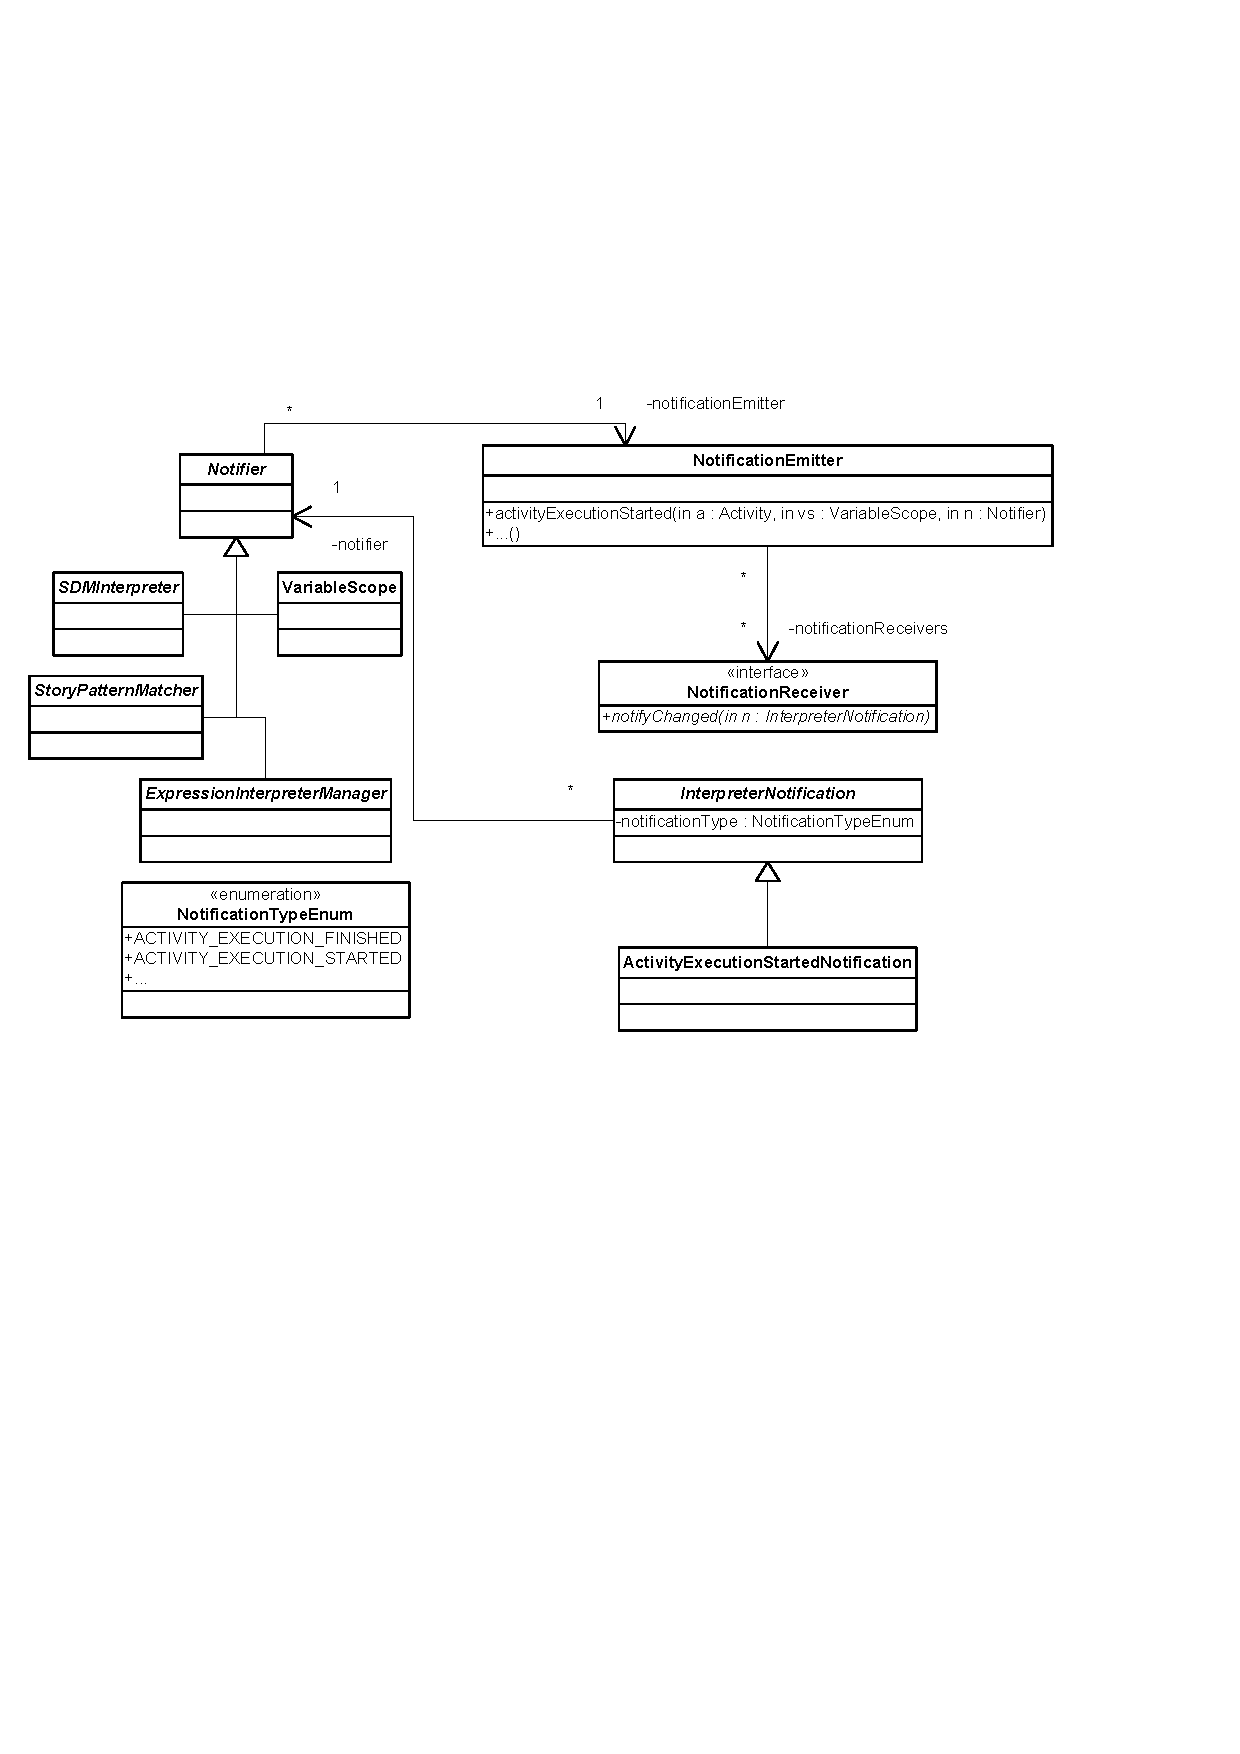
\includegraphics[width=1.0\columnwidth]{figures/interpreter_notification.pdf} 
\caption{Relevant classes of the interpreter's notification mechanism}
\label{fig:sdm_interpreter_notification}
\end{figure}

The interpreter and its subcomponents provide a notification mechanism to inform clients of all important steps during the execution of a story diagram.
This is an implementation of the observer design pattern.

\emph{SDMInterpreter}, \emph{StoryPatternMatcher}, \emph{VariableScope}, and \emph{ExpressionInterpreterManager} extend the \emph{Notifier} superclass, see Fig.~\ref{fig:sdm_interpreter_notification}.
\emph{Notifier} defines a reference to a \emph{NotificationEmitter}. 
This class provides an operation for each type of notification defined in \emph{NotificationTypeEnum} that creates an \emph{InterpreterNotification} and forwards it to all registered \emph{NotificationReceivers} by calling their \emph{notifyChanged()} operations. 
Clients can add their own \emph{NotificationReceiver}s to the \emph{NotificationEmitter}'s list of receivers.

By default, each \emph{Notifier} uses the default implementation in \emph{NotificationEmitter}. 
However, it is also possible to create \emph{Notifiers} with custom implementations of \emph{NotificationEmitter} to directly process notifications there or process notifications asynchronously, for example.


\subsection{Interpreting Story Diagrams}
\label{sec:sdm_interpreting}

\begin{figure}[htbp]
\center
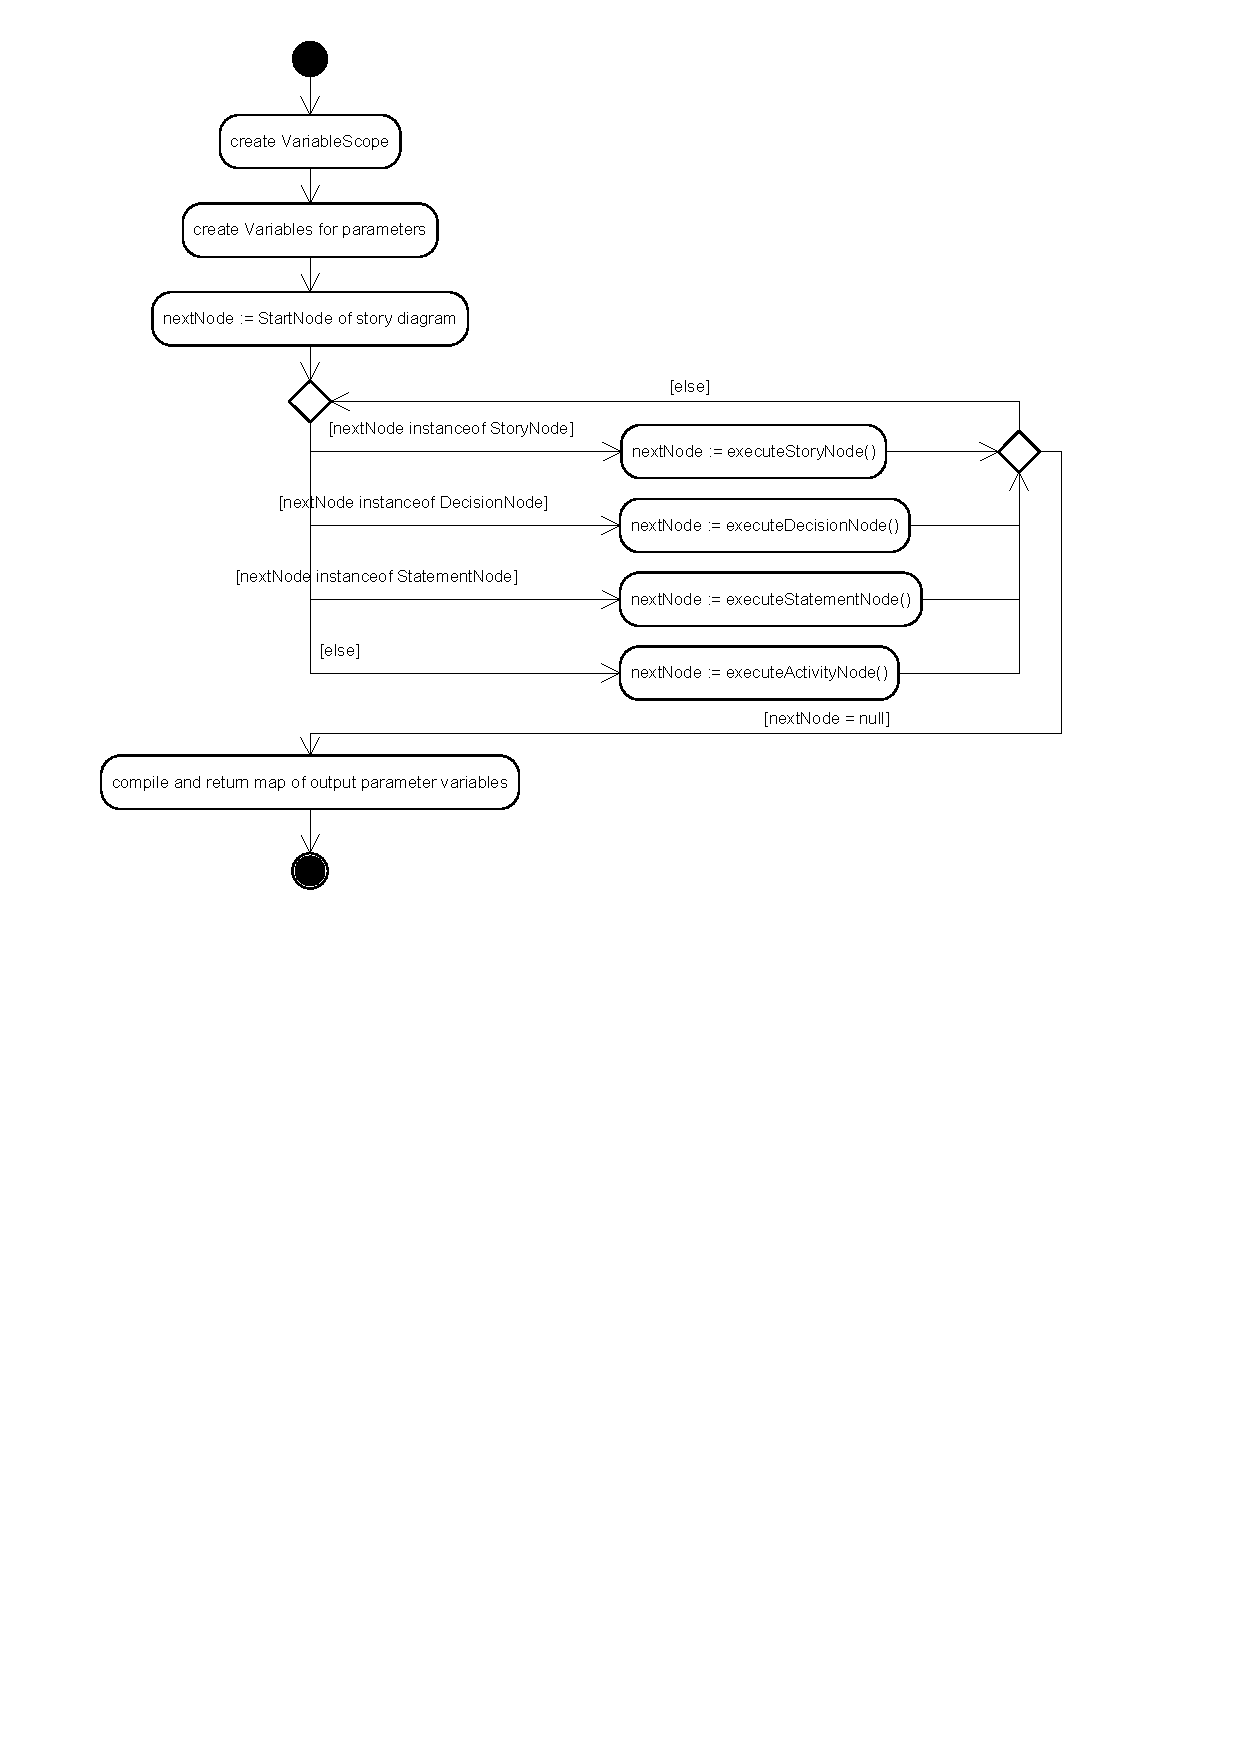
\includegraphics[scale=0.7]{figures/SDInterpreterExecution.pdf} 
\caption{Execution Scheme of the \emph{SDMInterpreter}}
\label{fig:sdmInterpreter_execution_scheme}
\end{figure}


The overall interpretation of a story diagram is a simple graph traversal algorithm.
The interpretation starts at the story diagram's \emph{StartNode} and traverses the story diagram until it reaches a \emph{StopNode}. 
All activity nodes are executed by specialized methods, which return the next activity node to execute afterwards. The activity diagram in Figure~\ref{fig:sdmInterpreter_execution_scheme} shows the overall execution scheme of the interpreter.

The interpreter is started with the \emph{executeActivity()} method.
This method creates the root \emph{VariableScope} and a \emph{Variable} for each parameter of the story diagram.
Then, the \emph{StartNode} of the story diagram is obtained and executed.

In general, the execution of activity nodes works as follows: 
First, the kind of the activity node is determined. Then, it is executed by the appropriate execution method.
\emph{StoryNode}s, \emph{JunctionNode}s, \emph{StopNode}s, and \emph{StatementNode}s require special handling by distinct execution methods.
All other kinds of activity nodes are skipped.
After execution of a node, the next node to execute is returned by the execution methods.
This process is repeated until a \emph{StopNode} is reached, which has no subsequent nodes.
Then, the loop terminates. The return value expressions of all outgoing parameters are evaluated and put into a map, which is returned by \emph{executeActivity()}.
This map maps the parameter names to their values.\footnote{For backward compatibility, all variables of the story diagram are currently returned, not only parameters.}

A non-for-each \emph{StoryNode} is executed using the \emph{StoryPatternMatcher} (cf. Section~\ref{sec:story_pattern_matcher}) with the \emph{DefaultMatchingStrategy}. 
It searches for a match of the story pattern and applies the graph transformation rule if a match was found. 
For for-each nodes, the process is more complex. 
If the story pattern is executed for the first time, a new \emph{StoryPatternMatcher} is created and stored in a local map for this \emph{StoryNode}. 
The pattern matcher is executed with the \emph{DefaultMatchingStrategyWithLog}, which keeps a log of the order in which elements were matched. 
If a match was found, the next activity node of the loop body is returned, i.e., that activity node that is connected to the for-each node via a for-each edge. 
The interpreter executes that node and eventually the control flow returns to the for-each node.
Now, the existing \emph{StoryPatternMatcher} is reused so that it continues pattern matching where it left off. 
This time, however, the pattern matcher uses the \emph{LogReproducingMatchingStrategy}. 
This ensures, that all elements are matched in the same order as the first time. 
For-each nodes are executed with the \emph{fresh match} semantics. 
After a match was found, the story pattern's side effects are executed immediately. 
Then, the next match is sought. 
Side-effects may influence subsequent matches, they may create new matches or eliminate existing ones. 
They may also influence they matching order if they change the number of elements in references, which changes the cost estimates (for details, see Section~\ref{sec:interpreting_story_patterns}). 
If the \emph{DefaultMatchingStrategy} would be used in each iteration of the for-each node, it may choose a different matching order in subsequent iterations. 
Due to the way how previous matches are managed, this may cause the pattern matcher to return a match multiple times or skip valid matches.
Therefore, the \emph{DefaultMatchingStrategyWithLog} is used in the first iteration of a for-each story node to log the matching order, and the \emph{LogReproducingMatchingStrategy} is used in all subsequent iterations, which matches elements in exactly the same order.

The stored mapping between the \emph{StoryNode} and the pattern matcher is discarded after the last loop iteration. 
If the story diagram's control flow returns to the for-each node again, the pattern matching process starts anew.

In addition to the \emph{fresh match} semantics, it is also possible to add other execution semantics for for-each nodes, e.g., \emph{pre-select}, which searches for all matches before executing side-effects.


\subsection{Interpreting Story Patterns}
\label{sec:interpreting_story_patterns}

The execution of a single story pattern comprises three steps:
Initialization of the pattern matcher and analysis of the story pattern (Section~\ref{sec:spm_initialization}),
pattern matching (Section~\ref{sec:spm_pattern_matching}),
and pattern application (Section~\ref{sec:spm_pattern_application}).
These steps are executed in the constructor of the pattern matcher, the \emph{findNextMatch()}, and the \emph{applyMatch()} operations respectively.
\emph{findNextMatch()} can be called successively to return all matches for a story pattern one-by-one.
These operations are separated, to allow for additional operations between these phases by the user of the pattern matcher.
The pattern matcher can also be used without the story diagram interpreter to execute a single story pattern.


\subsubsection{Initialization and Pattern Analysis}
\label{sec:spm_initialization}

A \emph{StoryPatternMatcher} is instantiated for a specific story pattern. 
Therefore, the \emph{StoryPatternMatcher}'s constructor already requires the story pattern as a parameter.
In the constructor, the matcher's internal data structures are set up. 
These comprise lists of the bound and unbound pattern variables\footnote{Subsequently, we use the term \emph{pattern variable} to refer to object variables or primitive variables in a story pattern in contrast to \emph{Variable}s to refer to \emph{Variable} objects used internally by the pattern matcher.}, checked and unchecked \emph{PatternPart}s, bound instance objects, the matching history, and the stack of match transactions.
The matching history is a mapping between pattern variables and lists of instance objects, that were previously bound to that pattern variable.
The match transaction stack is a stack that contains stack elements for each relevant action of the matcher.
Each time, a pattern part is matched or checked, or a pattern variable is bound to an object, a match transaction is executed and pushed onto the stack.
A transaction usually involves a manipulation of the internal data structures of the matcher, e.g., moving an element from the list of unbound to that of bound pattern variables.
When the matcher has to step back, these match transactions are popped from the stack and rolled back.
After initializing these data structures, the story pattern is divided into pattern parts as described in Sec.~\ref{sec:story_pattern_matcher}.
%Currently, each unconnected pattern variable and each link variable with its connected pattern variables form a pattern part.
%This implies that a single pattern variable may belong to multiple pattern parts.
%The matching process works on the granularity of these pattern parts.
%This is the current default semantics specific for the two introduced metamodels.
%This semantics can be different for other metamodels and it can be changed to support, e.g., complex negative application conditions.


\subsubsection{Pattern Matching}
\label{sec:spm_pattern_matching}

\lstset{
	numbers=left
}

\begin{figure}[htbp]
\begin{lstlisting}
create child variable scope of current variable scope;

bind bound objects;

check unchecked pattern parts;

boolean match = true;

do {
  while (nextPatternPart = 
      matchingStrategy.getNextPatternPart() != null) {
    
    commit matchPatternPart transaction;
    match = nextPatternPart.match();
    
    if (not match) {
      roll back last two matchPatternPart transactions;
      
      if (matchingStack is empty)
        break;
    }
  }
    
  if (match) {
    match = checkStoryPatternConstraints();
    if (not match)
      roll back last matchPatternPart transaction;
  }
} while (matchingStack is not empty and not match)

if (match) {
	merge child variable scope into its parent scope;
}
\end{lstlisting}
\caption{Overall pattern matching algorithm}
\label{listing:pattern_matcher_execution}
\end{figure}

\emph{findNextMatch()} is responsible for searching for the next valid match of the story pattern in the instance model.
The operation returns a boolean value indicating whether a match was found or not.
If a match was found, the pattern matcher's \emph{VariableScope} is manipulated accordingly.
If no match was found, the \emph{VariableScope} is left untouched.
Fig.~\ref{listing:pattern_matcher_execution} shows the overall scheme of this method.

First, a new variable scope is created, which is a child of the current variable scope.
During pattern matching, this child variable scope is modified but its parent is left untouched.
Next, all pattern variables that are marked as bound are bound to the appropriate variables in the \emph{VariableScope}.
Pattern variables with binding expressions are also handled here.
After that, all unchecked pattern parts are checked.
After binding all pattern variables, some pattern parts may contain only bound objects.
These pattern parts can be checked already at this point.
If a check fails, there can be no match for the story pattern and the pattern matcher terminates.
Otherwise, the actual pattern matching algorithm starts.

In two nested loops, the matching strategy returns the next pattern part to use for matching.
The matching strategy may use arbitrary heuristics to choose a pattern part from the list of unchecked pattern parts.
The default strategy returns that pattern part with the lowest cost estimate.
This pattern part must contain at least one bound and one unbound object and it must be possible to navigate from the bound objects to the unbound objects.
The \emph{calculateMatchingCost()} operation used in both metamodel specific implementations checks this.
A transaction for matching the current pattern part is pushed on the stack and the pattern part's \emph{match()} operation is called.
This operation is specific to the actual type of the link of the pattern.
In case of ordinary \emph{LinkVariables}, \emph{match()} simply follows the link from the bound instance object and tries to bind the unbound pattern variable to an instance object of the object graph.

If matching the pattern part was successful, i.e. \emph{match()} returned true, the loop continues with the next pattern part.
When all pattern parts have been matched, the matching strategy returns null instead of a pattern part.
Now, all constraints are checked that are defined for the whole story pattern.
If these conditions are also satisfied, a valid match has been found.
Now, the child variable scope is merged into its parent scope to persist the match, i.e. the \emph{Variable}s created for the matched objects are merged into the parent scope so that the caller of the pattern matcher can access the matched objects.

In case the \emph{match()} operation did not find a match, the last transactions including the one committed in line 13 of Fig.~\ref{listing:pattern_matcher_execution} for matching pattern parts have to be rolled back.
Of course, this also rolls back all bindings of pattern variables that were performed in the meantime.
Here, also the second last transaction has to be rolled back because the pattern variable matched in that transaction has now shown to be an invalid match and a new match has to be found for it.
A roll back is also performed if the constraints defined on the whole story pattern are not satisfied.
If a roll back leads to an empty matching stack, the pattern matching process is terminated because no valid match exists.


\subsubsection{Pattern Application}
\label{sec:spm_pattern_application}

After finding a match for a story pattern, the story pattern can be applied, i.e. its side-effects can be executed.
This is done in \emph{applyMatch()}, which must be called be the caller of the pattern matcher explicitly.
First, all attribute assignments are evaluated and their results are stored in a list.
After that, all objects marked as \destroy are deleted and then all links.
Finally, all objects and links marked for creation are created and all attributes are assigned their new values.

It is important that all objects are deleted before deleting any links.
Object deletion is performed via the \emph{EcoreUtil.delete()} operation, which also deletes all cross-references to the deleted object.
To do so, this operation walks the containment hierarchy upwards and searches for cross-links in the whole model tree.
If the pattern matcher would delete links first, it might not be possible to walk the containment hierarchy upwards if the deleted link pointed to the container of a deleted object.
Then, it would be impossible to delete all cross-references.

Attribute assignment expressions are evaluated at the beginning to support expressions that refer to deleted elements. 
If attribute assignments would be evaluated at the end, it would not be possible to evaluate expressions with references to deleted elements because these do not exist anymore in the \emph{VariableScope}.


%\section{Code Generation for Story Diagrams}
%As stated in the introduction of this chapter, a second possibility of executing story diagrams besides interpretation is code generation.
%When story diagrams were originally conceived, this was the first approach to executing them.
%The \fuj Tool Suite \cite{KNNZ99,NNZ00} provided the possibility to generate Java code from the story diagrams that could then be executed.
%This functionality was retained throughout several versions of \fuj and even extended to allow the generation of EMF-compatible code \cite{GBD07}.
%With the creation of the new metamodel for story diagrams \cite{HRvD+11}, this option was discontinued in favour of the interpretation described in Section~\ref{sec:InterpretingStoryDiagrams}.